\section{GREEDY framework}

\begin{Definition}
  Let $\mathcal{D}$ be the \defi{document array}{Document Array} of length $n$. For each suffix $\id{SA}[i]$ the document array $\mathcal{D}[i]$ contains the identifier of the document, in which suffix $\id{SA}[i]$ starts. A suffix array (or suffix tree) with this information added is called \defi{generalized suffix array}{Generalized Suffix Array} (or \defi{generalized suffix tree}{Generalized Suffix Tree}).
\end{Definition}

\begin{Definition}
  The \defi{GREEDY framework}{GREEDY Framework} for single term $f_{d,q}$-ranking of Culpepper et al. \cite{Culpepper2010} consists of:
  \begin{itemize}
    \item A compressed suffix array \id{CSA} of concatenation $\mathcal{D}$.
    \item A wavelet tree \id{WTD} of the document array of $D$.
  \end{itemize}
  The pseudocode \proc{Ranked-Search} for a query $q$ is given in Algorithm~\ref{alg:greedyRankedSearch}. The first step is a backward search in the compressed suffix array \id{CSA} to get the interval $[l,r]$ of all occurrences of $q$. This interval is stored in a priority queue. As long as this is not empty and we do not yet extracted $k$ documents, we take the longest interval from the priority queue. If this is a leave, we output its corresponding symbol as a hit. Otherwise we split the interval into the corresponding intervals of the two children in the wavelet tree \id{WTD}.
\end{Definition}

\begin{algorithm}[htb]
  \begin{codebox}
    \Procname{$\proc{Ranked-Search}(q, k)$}
    \li $[l,r] \gets \proc{Backward-Search}(CSA, q)$
    \li $\attribii{pq}{push}(\langle r - l + 1, [l,r], \attribii{WTD}{root}()\rangle)$ \>\>\>\>\>\>\>\>\Comment Max-PQ sorted by interval size.
    \li $h \gets 0$
    \li \While $h < k$ and not $\attribii{pq}{empty}()$
        \Do
    \li   $\langle s, [l,r], v \rangle \gets \attribii{pq}{pop}()$
    \li   \If \attribii{WTD}{is\_leaf}()
          \Then
    \li     \textbf{output} $\langle \attribii{WTD}{symbol}(v) \rangle$
    \li     $h \gets h + 1$
    \li   \Else
    \li     $\langle \langle [l_l, r_l], v_l \rangle \langle [l_r, r_r], v_r \rangle \rangle \gets \attribii{WTD}{expand}(v, [l,r])$
    \li     $\attribii{pq}{push}(\langle r_l - l_l + 1, [l_l, r_l], v_l \rangle)$
    \li     $\attribii{pq}{push}(\langle r_r - l_r + 1, [l_r, r_r], v_r \rangle)$
          \End
        \End
  \end{codebox}
  \caption{Search for top-$k$ documents containing $q$.}
  \label{alg:greedyRankedSearch}
\end{algorithm}

\begin{Example}
  Consider the text $T = \omega_2\omega_1\omega_3\omega_3\#\omega_1\omega_1\omega_4\omega_1\#\omega_1\omega_4\omega_3\omega_1\#\omega_5\omega_5\#$ with $\# < \omega_1 < \ldots < \omega_5$. The suffix array is $\id{SA} = \{4,9,14,17,{\color{red}8,13,5,6,1,10},12,0,3,2,7,11,16,15\}$ and the document array is $\mathcal{D} = \{0,1,2,3,{\color{red}1,2,1,1,0,2},2,0,0,0,1,2,3,3\}$. The red parts are the range \proc{Backward-Search} returned for query $\omega_1$. The interval in $\mathcal{D}$ corresponds to the multiset of all documents containing $\omega_1$. Figure~\ref{fig:greedyWaveletTree} shows the wavelet tree over $\mathcal{D}$ with the interesting intervals marked in red. The leave intervals are extracted in order $1,2,0$. So for a top-$2$-query, we would have found $d_1$ ($3$ occurrences) and $d_2$ ($2$ occurrences).

  \begin{figure}[htb]
    \centering
    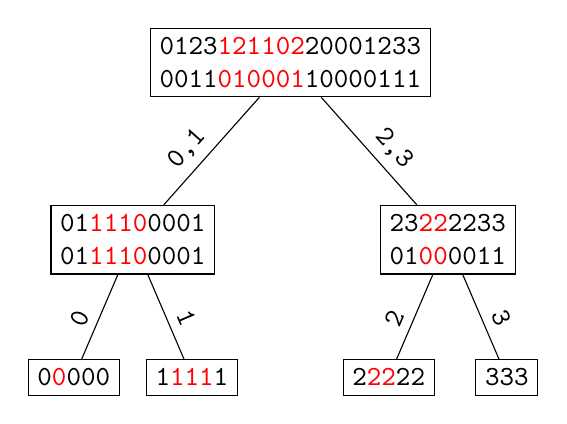
\begin{tikzpicture}[every text node part/.style={align=center}]
  \node[draw] (0) at (0,0) {\texttt{0123{\color{red}121102}20001233}\\\texttt{0011{\color{red}010001}10000111}};
  \node[draw] (1) at (-2,-2.25) {\texttt{01{\color{red}1110}0001}\\\texttt{01{\color{red}1110}0001}};
  \node[draw] (2) at (2,-2.25) {\texttt{23{\color{red}22}2233}\\\texttt{01{\color{red}00}0011}};
  \node[draw] (3) at (-2.75,-4) {\texttt{0{\color{red}0}000}};
  \node[draw] (4) at (-1.25,-4) {\texttt{1{\color{red}111}1}};
  \node[draw] (5) at (1.25,-4) {\texttt{2{\color{red}22}22}};
  \node[draw] (6) at (2.75,-4) {\texttt{333}};

  \draw (0) -- (1) node[above, sloped, pos=0.6] {\texttt{0,1}};
  \draw (0) -- (2) node[above, sloped, pos=0.6] {\texttt{2,3}};
  \draw (1) -- (3) node[above, sloped, pos=0.6] {\texttt{0}};
  \draw (1) -- (4) node[above, sloped, pos=0.6] {\texttt{1}};
  \draw (2) -- (5) node[above, sloped, pos=0.6] {\texttt{2}};
  \draw (2) -- (6) node[above, sloped, pos=0.6] {\texttt{3}};
\end{tikzpicture}

    \caption{The wavelet tree over the document array $\mathcal{D}$. The interval with the documents corresponding to query $q = \omega_1$ are marked in red.}
    \label{fig:greedyWaveletTree}
  \end{figure}
\end{Example}

\begin{Theorem}
  The GREEDY framework needs time $\mathcal{O}(N \cdot(t_{deleteMax} + t_{insert}))$ in the worst case, where $N$ is the number of documents in the collection and $t_{deleteMax}$ and $t_{insert}$ are the times needed for the corresponding wavelet tree operations.
\end{Theorem}

\begin{Proof}
  Consider a collection $\mathcal{D}$ where each $d \in \mathcal{D}$ is the same, for example $d = a$. Let the query be $a$ as well.

  The backward search will return the whole set of all documents (excluding the sentinels), because every document contains the query. Not the GREEDY framework steps through the wavelet tree until $k$ leaves are found. In each step it takes the biggest interval from the priority queue and inserts its two children. Since the intervals in the leaves are of size $1$ each, first all inner nodes must be processed. For $N$ documents in the wavelet tree there are $N-1$ inner nodes. Therefore the runtime is $\mathcal{O}(N \cdot(t_{deleteMax} + t_{insert}))$.
\end{Proof}
